\documentclass{beamer}


%\includeonlyframes{compconv}
%\includeonlyframes{approach}
%\includeonlyframes{res}
%\includeonlyframes{overview,overviewn,deriv,dual,subgrad,intro}
\mode<presentation>

\usepackage{tikz}
\usepackage{tikz-qtree}

\usetikzlibrary{arrows}
\usetikzlibrary{automata}
\usetikzlibrary{positioning}
\usetikzlibrary{shapes,snakes}

\title{Tracking and Visualizing \\ Provenance using PostgreSQL}
\author{Nirmesh Malviya and Alexander Rush}
\begin{document}

\begin{frame}
\titlepage
\end{frame}

\begin{frame}{What is Provenance?}
  \begin{itemize}
  \item \textbf{Provenance} - where data comes from, how it was derived, manipulated, and combined, and how it has been updated over time.
  \item \textbf{Data Provenance} - pertains to the derivation history of a data product starting from its original sources.
  \item Motivation
    \begin{itemize}
    \item Scientific Data - Maintain consistency with raw data
    \item Business Apps - Synchronize data with third parties
    \end{itemize}
    
  \end{itemize}
\end{frame}

\begin{frame}{Storing Provenance}
  \begin{figure}
  \centering
  \label{diag}


  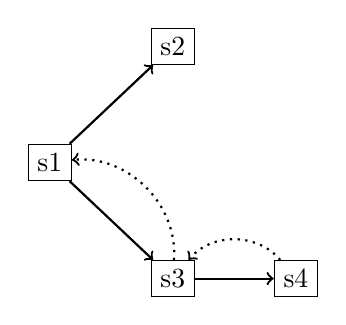
\begin{tikzpicture}
    \node (s1) [draw]{s1};

    \node (s2) [draw,above right= of s1]{s2};
    \node (s3) [draw,below right= of s1]{s3};
    \node (s4) [draw, right= of s3]{s4};
    \path [->] (s1) edge[thick] (s2);    
    \path [->] (s1) edge[thick] (s3);    
    \path [->] (s3) edge[thick] (s4);    

    \path [->] (s4) edge[thick, bend right = 50, dotted] (s3);    
    \path [->] (s3) edge[thick, bend right = 50, dotted] (s1);    
  \end{tikzpicture}
  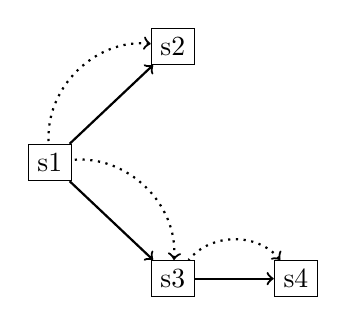
\begin{tikzpicture}
    \node (s1) [draw]{s1};

    \node (s2) [draw,above right= of s1]{s2};
    \node (s3) [draw,below right= of s1]{s3};
    \node (s4) [draw, right= of s3]{s4};
    \path [->] (s1) edge[thick] (s2);    
    \path [->] (s1) edge[thick] (s3);    
    \path [->] (s3) edge[thick] (s4);    

    \path [<-] (s4) edge[thick, bend right = 50, dotted] (s3);    
    \path [<-] (s3) edge[thick, bend right = 50, dotted] (s1);    
    \path [<-] (s2) edge[thick, bend right = 50, dotted] (s1);    
  \end{tikzpicture}

  \caption{ (b) Backward provenance (a) Forward provenance}

\end{figure}

\end{frame}

\begin{frame}{Provenance in Postgres }
   \begin{center}
  \scalebox{0.6} {
    
      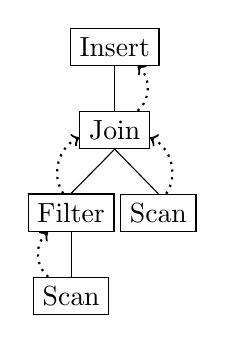
\begin{tikzpicture}
        \Tree [ .\node[draw, rectangle](i1){Insert}; [ .\node[draw, rectangle](j1){Join}; [ .\node[draw, rectangle] (f1) {Filter};  
        \node[draw, rectangle](s1){Scan}; ]  \node[draw, rectangle] (s2) {Scan};  ] ]   

        \path [->] (s2) edge[thick, bend right = 50, dotted] (j1);    
        \path [->] (s1) edge[thick, bend left = 50, dotted] (f1);            
        \path [->] (j1) edge[thick, bend right = 50, dotted] (i1);    
        \path [->] (f1) edge[thick, bend left = 50, dotted] (j1);    
        
      \end{tikzpicture}
    }
  \end{center}
  \begin{itemize}
  \item Added catalog table \texttt{pg\_prov} to store provenance graph.
  \item Modified Postgres execution engine to track provenance along the query execution tree.
  \item Made changes to storage engine to maintain data provenance of intermediate tuples written to disk during execution. 
  \item Supports filters, subqueries, joins, aggregates, order by, and group by. 
  \end{itemize}
\end{frame}

\begin{frame}{Demo}
  \begin{figure}
  \centering

  \includegraphics[scale=0.3]{prov.png}
  \caption{ Provenance graph}
  
\end{figure}

\end{frame}


\end{document}